\iffalse
\begin{itemize}
	\item Initial state construction (State Identification)
	\item Aggregation (State Aggregation)
	\item Transition probabililties (Modeling transitions)
\end{itemize}
\fi

To capture and summarize the dynamics of the system our methodology represents the data
in a qualitative manner using states and transitions. We begin this section with an overview
of our multi-scale methodology. The methodology consists of three main steps and is
shown in Figure \ref{fig:methodology}.

\begin{figure}[h!]
	\centering
	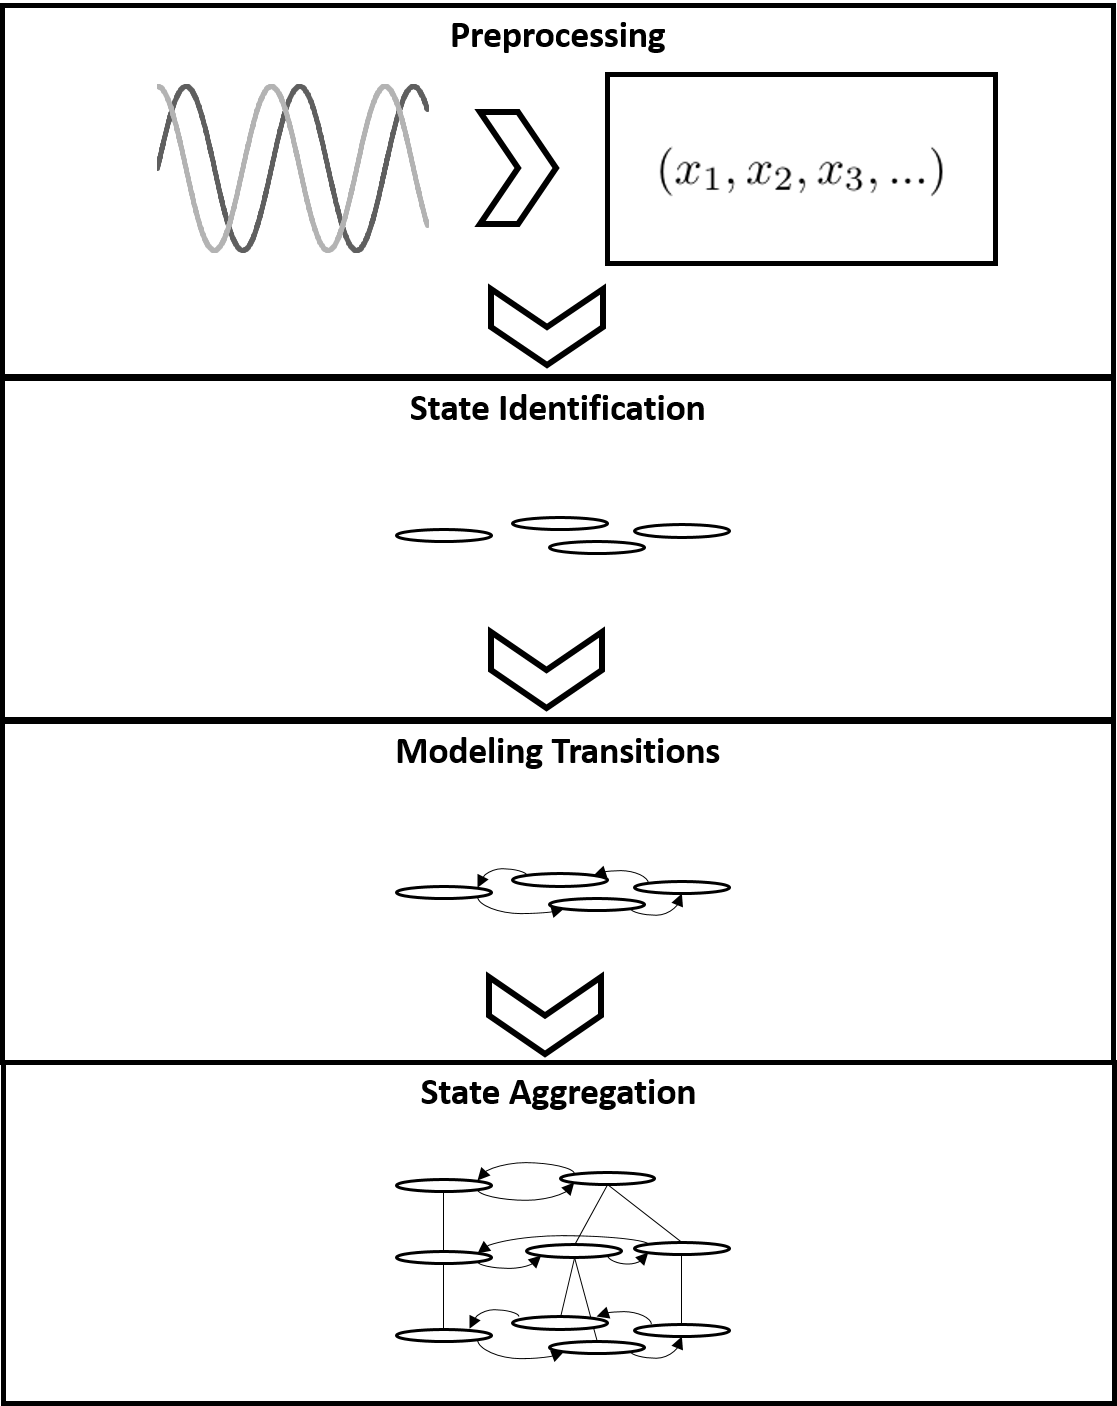
\includegraphics[width=\columnwidth]{methodology}
	\caption{\lstopar{TODO}}
	\label{fig:methodology}
\end{figure}
The methodology starts in the top left part of the figure with an initial step that summarizes
the structure of the data by identifying their most typical states. It achieves this by \lstopar{placing}
the data in a \lstopar{design time} metric space and partitioning them. It then associates
each partition with a single state.
\lstopar{
\begin{itemize}
	\item These states are used as the lowest-level states.
\end{itemize}
}
The methodology then moves in the counter clockwise direction. The second step summarizes
dynamics. It does so using the continuous time Markov chain framework presented in Section \ref{sec:preliminaries}.
The third and final step aggregates states and transitions into a hierarchy, associating each
level of the hierarchy with a unique scale, thus providing a multi-scale model. These steps 
are explained in detail in the next subsections.


\subsection{Initial State Construction}
\label{sec:framework-states}

The first step in our methodology is the construction of initial lowest level states. Using the notation
from Section \ref{sec:preliminaries} we define a partition function 
from $\lstopar{f}: \mathbb{R}^d \rightarrow I$ mapping the $d$-dimensional signal to lowest level states
\lstopar{
with the following properties:
\begin{itemize}
	\item similar points in $\mathbb{R}^d$ should be mapped to the same or neighboring partitions.
\end{itemize} 
}

\subsection{Modeling Transition Probabilities}
\label{sec:framework-transitions}

While we represent the states as described in Section \ref{sec:framework-states},
to model transitions we use the continuous-time Markov chain (CTMC) framework.
As mentioned in Section \ref{sec:preliminaries} all the data needed to represent a continuous-time Markov chain
is stored as transition rates in a transition rate matrix $Q \in \mathbb{R}^{n \times n}$, where $n$ represents
the size of the finite state space $I$. However, initial user
feedback showed transition rates are not a very informative way of visualizing state transitions. Therefore
we choose to visualize transitions in terms of the jump chain $\Pi$.
We note that an alternative way of representing a Markov chain $(X_t)_{t \ge 0}$ with transition rate matrix $Q$
is by its jump chain and holding times. The jump chain of a continuous time Markov chain $(X_t)_{t \ge 0}$ is
a discrete time Markov chain $(Y_n)_{n \ge 0}$ with transition matrix $\Pi$ defined as
\begin{equation}
	\nonumber
	\left(\Pi\right)_{ij} = 
		\left\{
			\begin{array}{ll}
				-\frac{q_{ij}}{q_{ii}} & \mbox{if } i \ne j, q_{ii} \ne 0 \\
				0 & \mbox{if } i \ne j, q_{ii} = 0
			\end{array}
		\right.
\end{equation}
\begin{equation}
	\nonumber
	\left(\Pi\right)_{ii} = 
		\left\{
			\begin{array}{ll}
				0 & \mbox{if } q_{ii} \ne 0 \\
				1 & \mbox{if } q_{ii} = 0
			\end{array}
		\right.
\end{equation}
Definition \ref{def:jump-chain-holding-times} provides a definition of a Markov chain in terms of its jump chain and holding times.

\begin{defn}
	\label{def:jump-chain-holding-times}
	A right-continuous process $(X_t)_{t \ge 0}$ is a continuous time Markov chain with initial
	distribution $\lambda$ and transition rate matrix $Q$ if its jump chain $(Y_n)_{n \ge 0}$ is a 
	discrete time Markov chain with initial distribution $\lambda$ and transition matrix $\Pi$ and
	for each $n \ge 1$, conditional on $Y_0, Y_1, ..., Y_{n-1}$, its holding times $S_1, S_2, ..., S_{n-1}$
	are independent exponentially distributed random variables of parameters $q_{Y_0}, q_{Y_1}, ..., q_{Y_{n-1}}$
	where $q_i = -q_{ii}$.
\end{defn}

To determine the size of each state, we turn to the ergodic properties of $(X_t)_{t \ge 0}$, specifically
we use the elements of the stationary distribution $\pi = (\pi_1, \pi_2, ..., \pi_n)$ and draw the area of
state $i$ proportional to $\pi_i$. We note that under the assumption presented in \ref{sec:preliminaries}
this distribution always exists.

\subsection{Aggregation}
\label{sec:framework-aggregation}

By the final step of our methodology, we have already computed a qualitative representation of the
dataset. The goal of the third step is then to construct a multi-scale representation, representing
the data in several details level - from the finest to the most coerce.

As stated in Section \ref{sec:preliminaries} we associate each scale $s$ with a specific partition
function $\lstopar{f_s}: \mathbb{R}^d \rightarrow \lstopar{I_s}$. At the finest scale, we use the 
partition function \lstopar{$f: A \rightarrow B$ [TODO the function]} as defined in Section \ref{sec:framework-states}, inducing state space $I$. We then compute the partition
function for coarser scales by aggregating elements in $\Ima \lstopar{f}$, inducing state space $I_s$.
Thus $I_s$ represents a partition of $I$.

\newpage

Once we have computed the lowest level Markov chain $(X_t)_{t \ge 0}$, we need to be able to represent it on multiple scales.
As stated in Section \ref{sec:preliminaries} we associate each scale $s$ with a specific partition function
$\lstopar{f_s}: \mathbb{R}^d \rightarrow \lstopar{I_s}$ where coarser partitions are generated by merging 
states of finer partitions.
Suppose we have already computed the finest level partition $\lstopar{\cP}$, inducing state space $I$ and the
coarser partition at scale $\lstopar{\cP_s}$, inducing state space $J$. Suppose the finest level Markov chain,
on state space $I$ is represented by a transition rate matrix $Q$ and define a surjective partition function
$\phi: I \rightarrow J$. To compute the Markov chain induced by state space $J$, we adapt a formula proposed
in \cite{5746509} to continuous time Markov chains. We define a \lstopar{transition rate matrix transformation function}
$\Phi: \mathbb{R}^{n \times n} \rightarrow \mathbb{R}^{m \times m}$ using formula \ref{eq:ctmc-state-aggregation}.
\begin{equation}
	\label{eq:ctmc-state-aggregation}
	\Phi(Q) = \tilde{Q} = (P' \Pi P)^{-1} P' \Pi Q P
\end{equation}
where $\Pi = diag(\pi)$ and $\pi = (\pi_1, \pi_2, ..., \pi_n)$ is the stationary distribution of $(X_t)_{t \ge 0}$, while $P$ is a 
$|I| \times |J|$ partition matrix with elements
\begin{equation}
	\nonumber
	\left(P\right)_{ij} = 
		\left\{
			\begin{array}{ll}
				1 & \mbox{if } \phi(i) = j \\
				0 & \mbox{otherwise}.
			\end{array}
		\right.
\end{equation}
If we define $\psi = \phi \circ \phi$, then Equation \ref{eq:ctmc-state-aggregation} can be rewritten as
\begin{equation}
	\nonumber
	\tilde{q}_{\phi(i)\phi(j)} = \frac{\sum\limits_{i \in \psi(i)}\pi_i \sum\limits_{j \in \psi(j)} q_{ij}}{\sum\limits_{i \in \psi(i)}\pi_i}
\end{equation}